\documentclass{report}
\usepackage[utf8]{inputenc}
\usepackage[english]{babel}
\usepackage{url}
\usepackage[hidelinks]{hyperref}
\usepackage{graphicx}
\usepackage{float}
\usepackage{booktabs}
\title{Homework 3\\ Electricity supply and solar cells}
\date{\today}
\author{Johanna Sörbom}

\newcommand{\case}[1]{\subsubsection*{#1}}
\newcommand{\ac}{AC-system}
\newcommand{\cmp}[2]{\ensuremath{#1+#2i}}
\newcommand{\mypart}[2]{\section*{Part #1 - \textit{#2}}}
\newcommand{\mysubpart}[1]{\subsection*{#1}}
\begin{document}
\maketitle
\chapter*{Introduction}
Someone wants to install solarcells on the roof of buildings in three areas in Sweden. In this report we are looking into how much sollarcells it is possible to install and what the profit would be if you did this. Would it be worth doing from an economic perspective? And what would happen if a dark cloud passed over the areas?

\section*{Method}
Through values given in the homework and excell answers to questions in this report has been answered. Information  has also been collected from relevant websites. 

\section*{Background}
The level of greenhouse gases in the atmosphere is today the highest that it has ever been. Since 1880 the averrage temperature has risen by $ 0.85 degees C $,. The greenhouse gasses emitted by humans are a big reason for this climate change and it is more and more important to change to renewable energy sources such as solar energy. (United Nations. 2017)

Solar energy is a renewable energysource that can be transformed into electricity. The energy that comes from the sun to earth is approximatly $ 15000 $ times as much as the total energy use in the world today. If only a bit of this could be harvested it could solve a lot of the worlds energy problems. (Vattenfall. 2016) That is why this report looks into the use of solar energy in three areas in Sweden to see if it would be profitable to use as a source for energy. 

\chapter*{Result and calculations}
\mypart{A}{What is the maximum possible income per year of building solar cells in the three areas of Brytpunkten, Framtiden and Solsidan?}
To find the maximum possible income per year by build solar cells you need to calculate the maximum square meters of solar cells possible to build in each of the three areas, Brytpunkten, Framtiden och Solsidan. While doing this the voltage have to stay between 63-77 kW and you also need to have the same amount of solar cells in each area. To help with these calculations an excell file was given in the assignment. The first step to solve this is to calculate the impendance of the power lines and add the results to the excell file.  After that the reactive power was calculated and added to the same excell file. By running the excell file with and without wind power active and without solar cells results on the voltage at Brytpunkten, Framtiden och Solsidan where attained. Se part \ref{Voltage1} for results.  

\mysubpart{Impedance of power lines}
The impedence of the power line is given by the equation 

\begin{equation}\label{eq_impd}
Z =  L \cdot Z_{km}
\end{equation} where $L$ is the length of the power line in kilometers and $Z_{km}$ is the impedience per kilometer in Ohms.

\case{Ställverket to Brytpunkten}
For the case of Ställverket to Brytpunkten, we have $L=10km$ and $Z_{km}=\cmp{0.2}{0.4}$.  We get,

\begin{eqnarray}
Z&=&  L \cdot Z_{km} \\
&=&10 (\cmp{0.2}{0.4}) \\
&=& \cmp{2}{4} \label{res1}
\end{eqnarray} by substituing into equation \ref{eq_impd}. Interpreting the real part of the result obtained in equation \ref{res1} as resistance and the complex part as reactance, we have $R=2\Omega$ and $X=4\Omega$ respectively.

\case {Brytpunkten to Framtiden}
For the case of Brytpunkten to Framtiden, we have $L=15km$ and $Z_{km}=\cmp{0.2}{0.4}$.  We get,

\begin{eqnarray}
Z&=&  L \cdot Z_{km} \\
&=&15 (\cmp{0.2}{0.4}) \\
&=& \cmp{3}{6} \label{res2}
\end{eqnarray} by substituing into equation \ref{eq_impd}. Interpreting the real part of the result obtained in equation \ref{res2} as resistance and the complex part as reactance, we have $R=3\Omega$ and $X=6\Omega$ respectively.

\case {Brytpunkten to Solsidan}
For the case of Brytpunkten to Solsidan, we have $L=21.21km$ and $Z_{km}=\cmp{0.2}{0.4}$.  We get,

\begin{eqnarray}
Z&=&  L \cdot Z_{km} \\
&=&21.21 (\cmp{0.2}{0.4}) \\
&=& \cmp{4.24}{8.49} \label{res3}
\end{eqnarray} by substituing into equation \ref{eq_impd}. Interpreting the real part of the result obtained in equation \ref{res3} as resistance and the complex part as reactance, we have $R=3\Omega$ and $X=6\Omega$ respectively.

\case {Framtiden to Solsidan}
For the case of Framtiden to Solsidan, we have $L=15km$ and $Z_{km}=\cmp{0.3}{0.1}$.  We get,

\begin{eqnarray}
Z&=&  L \cdot Z_{km} \\
&=&15 (\cmp{0.3}{0.1}) \\
&=& \cmp{4.5}{1.5} \label{res4}
\end{eqnarray} by substituing into equation \ref{eq_impd}. Interpreting the real part of the result obtained in equation \ref{res4} as resistance and the complex part as reactance, we have $R=4.5\Omega$ and $X=1.5\Omega$ respectively.

\case {Vindeby to Solsidan}
For the case of Vindeby to Solsidan, we have $L=15km$ and $Z_{km}=\cmp{0.3}{0.1}$.  We get,

\begin{eqnarray}
Z&=&  L \cdot Z_{km} \\
&=&15 (\cmp{0.2}{0.4}) \\
&=& \cmp{3}{6} \label{res5}
\end{eqnarray} by substituing into equation \ref{eq_impd}. Interpreting the real part of the result obtained in equation \ref{res5} as resistance and the complex part as reactance, we have $R=3\Omega$ and $X=6\Omega$ respectively.

\mysubpart{Reactive power}
Complex power is defined as, \begin{equation}
S = \sqrt{P^2 - Q^2} \label{s}
\end{equation}
where $P$ is the active power and $Q$ is the reactive power. For balanced load in an \ac we have, 
\begin{equation}
P = S \cdot \cos\theta
\end{equation}
where $\theta$ is the phase offset between voltage and current. 

\case{Brytpunkten}
For the case of Brytpunkten where $\cos\theta = 0.9$ and $P = 35 MW$ we get,
 
\begin{eqnarray}
Q&=&   = \sqrt{S^2 - P^2}\\
&=& \sqrt{38.89^2 - 35^2} \\
&=& 16.95 MW \label{res}
\end{eqnarray} 
by substituting into equation \ref{s}.

\case{Framtiden}
For the case of Framtiden where $\cos\theta = 0.9$ and $P = 10 MW$ we get,
 
\begin{eqnarray}
Q&=&   = \sqrt{S^2 - P^2}\\
&=& \sqrt{11.11^2 - 10^2} \\
&=& 4.84 MW \label{res}
\end{eqnarray} 
by substituting into equation \ref{s}.

\case{Solsidan}
For the case of Solsidan where $\cos\theta = 0.9$ and $P = 5 MW$ we get,
 
\begin{eqnarray}
Q&=&  \sqrt{S^2 - P^2}\\
&=& \sqrt{5.56^2 - 5^2} \\
&=& 2.43 MW \label{res}
\end{eqnarray} by substituting into equation \ref{s}.

\mysubpart{Voltage in power lines}\label{Voltage1}
By using Excell to calculate the voltage in the power lines using data from above we get two cases.

\case{Not using wind power or solar power}
Not using wind power or solar power results in the following voltage in the power lines. 

\begin{table}[H] 
\begin{tabular}{ll}
\toprule
Location & Voltage (kV) \\
\midrule
Brytpunkten & 67.00\\
Framtiden  &  66.18\\
Solsidan & 66.26\\
\bottomrule
\end{tabular} 
\end{table} 

As seen in figure \ref{fig_utan_vindeby}
\begin{figure}[h]
\label{fig_utan_vindeby}
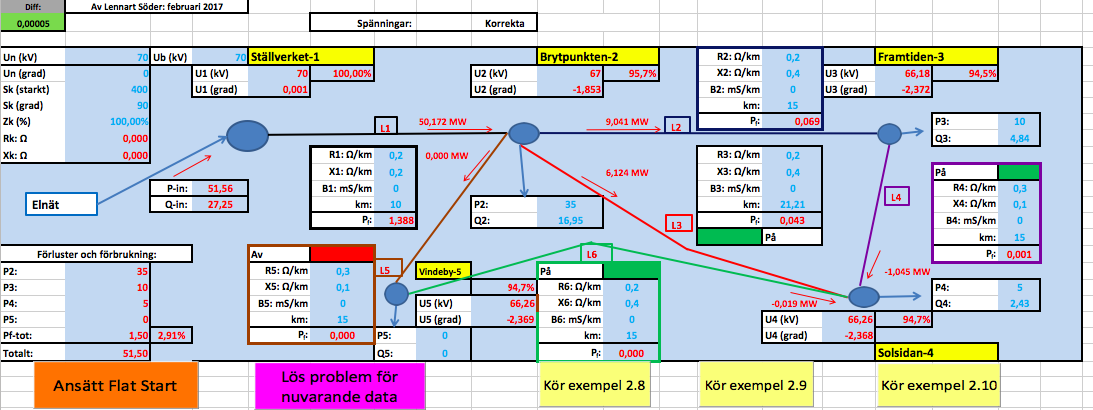
\includegraphics[width=\linewidth]{utan_vindeby.png}
\caption{Voltage when using wind power from Vindeby.} 
\end{figure}

\case{Using wind power but not solar power}
Using wind power but not solar power results in the following voltage in the power lines, 

\begin{table}[H] 
\begin{tabular}{ll}
\toprule
Location & Voltage (kV) \\
\midrule
Brytpunkten & 65.72 \\
Framtiden  &  64.15\\
Solsidan & 63.5\\
\bottomrule
\end{tabular} 
\end{table}

As seen in figure \ref{fig_med_vindeby}
\begin{figure}[h]
\label{fig_med_vindeby}
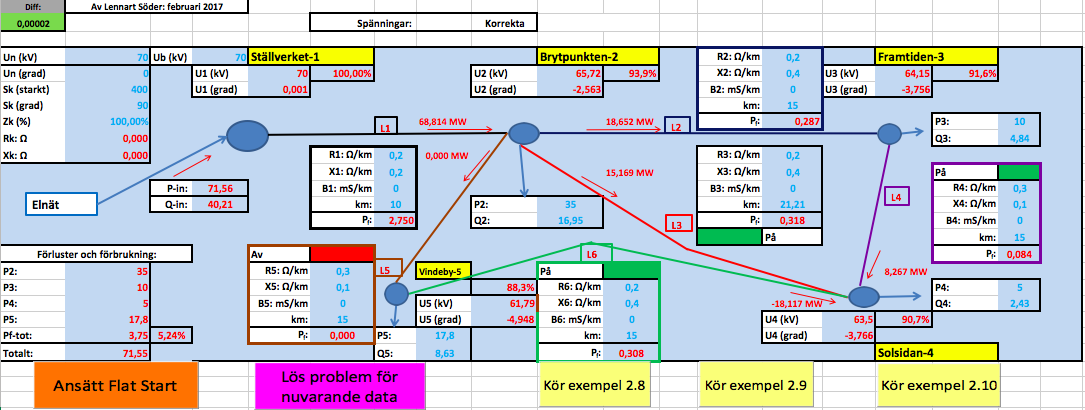
\includegraphics[width=\linewidth]{med_vindeby.png}
\caption{Voltage when not using wind power.} 
\end{figure}

\mysubpart{Total area of solar cells possible }
To find the maximum square meters of solar cells possible at each area without making the voltage in the power lines at each area to high or to low, we lower the active effect until the voltage is either over 77 or under 63. In this case the solar panels supply effect to the buildings and they need less from the rest of the power grid. By doing this in even steps a result was attained when the voltage at Solsidan became to high. This occurred after lowering the power with 96MW. That means that the total capacity for solar energy in the three areas is, 
\begin{equation}
P = 3 \cdot 96 = 288MW
\end{equation}

This is an area of,
\begin{eqnarray}
A&=&  P/\eta \cdot E_{sol}/m^2 \cdot 10^{-3} \\
&=& 288 \cdot 10^6 / 0.18 \cdot 1 \cdot 10^{-3} \\
&=&  1600000 m^2}
\end{eqnarray}

\begin{figure}[h]
\label{voltagechange}
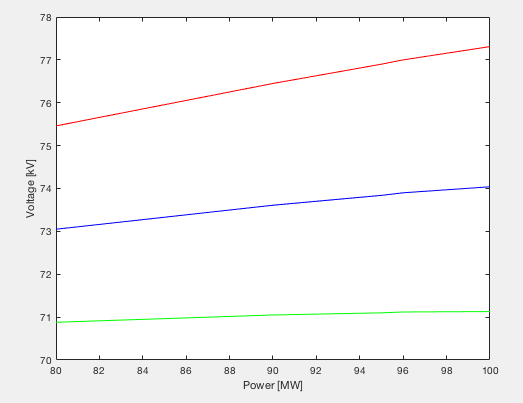
\includegraphics[width=\linewidth]{voltagechange.png}
\caption{Voltage change when installing solar cells where green is Brytpunkten, blue is Framsidan and Red is Solsidan.} 
\end{figure}

 
\mysubpart{ Maximum possible income}
The income for solar cells is $ 1.316 kr/kWh $ every kW solar cells produce 1000 kWh/year and we can build $  $ of solar cells. This gives a maximum yearly income of, 
\begin{equation}
I = 288 \cdot 10^6 \cdot 1.316 = 379008000 kr
\end{equation}

\newpage 
\mypart{B}{Is building the solar cells from question A economically viable?}

Income for installing solar cells come from a number of factors. These are electricity sales, electricity certification,  GOO-Guaranties of Origin and tax-reduction.

\mysubpart{Electricity sales}
Nordpool controls the prices of the electricity being sold. In this report the price of electricity is assumed to be the average year 2010 for the months of August and October. 

\begin{equation}
August = 0.417 kr/kWh
\end{equation}

\begin{equation}
October = 0.495 kr/kWh
\end{equation}

\begin{equation}
Price electricity = ( 0.417  + 0.495)/2 = 0.456 kr/kWh
\end{equation}

\mysubpart{Electricity certification}
Electricity certification is a support system to encourage increased production of renewable electricity. According to Nasdaq certificates where sold to Electricity Nordic Future for $ 0.26 kr/kWh$. (Nasdaq. 2017)

\mysubpart{GOO-Guaranties of Origin}
At the EEX Goos can be purchased for $ 0.00008 kr/kWh $. (European Energy Exchange. 2017)


\mysubpart{Tax-reduction.}
As from the 1 of January 2015 excess electricity can be pumped into the national powergrid for a taxreduction. The tax reduction is $ 0.6 kr/kWh $ with a maximum of the amount of hour previously purchased from the powergrid or $ 30 000 kWh $. In this report every kWh of solar energy gives an income of $ 0.6 kr $. 

\mysubpart{Profit}
Adding all of these incomes gives a total income of $ 1.316 kr/kWh $. Havin solar cells cost 1 kr/kWh. This means a profit of, 
\begin{eqnarray}
Profit&=& Income - cost \\
&=& 1.316 - 1 \\
&=& 0.316 kr/kWh}
\end
Building $ 288 m^2 $ of solar cells is profitable. 

\mypart{C}{Is it economically viable to build a parallel power line to strengthen the power lines and be able to increase the number of solar cells?}

Building a parallel power line to strengthen the power lines means that they can take a higher voltage and therefore transport more electricity. This makes it possible to install more solar cells at the different areas. A way of strengthening the power lines is to lower the impediance by make them thicker and making the isolation better.

The investment cost to build an additional power line with voltage $ 70 kV $ is $ 1 800 000 kr/km $. In part A we got the result that the power line at Solsidan is the limiting power line and therefore the one that might profit from an additional power line. To decide weather to add an additional  additional power line between Brytpunkten and Solsidan or between Framtiden and Solsidan the impedance is divided by two and a new voltage attained. We want to build the power line at the place where we get the highest voltage. This turns out to be between Brytpunkten and Solsidan.

\mysubpart{Brytpunkten to Solsidan }
The current power line between Brytpunkten and Solsidan has the impedance,
\begin{equation}
Z = \cmp{0.2}{0.4} 
\end{equation}

Strengthening this power line means cutting the impedance in half, \begin{equation}
Z = \cmp{0.1}{0.2} 
\end{equation}

The length of this power line is $ 21.21 km $ which means it the cost of building the additional power line here is, 
\begin{equation}
Cost = 21.21 \cdot 1800000 = 38178000 kr 
\end{equation}

Running the excell file with the new values and finding where the voltage is no longer in the range 63-77 a new maximum capacity for of solar cells can be calculated. This happens at Framtiden and we can now install $ 155 MW $ solar cells in each area.\\

\begin{equation}
P = 3 \cdot 155 = 465 MW
\end{equation}

The profit of having solar cells is as seen in part B,
\begin{eqnarray}
Profit&=& Income - cost \\
&=& 1.316 - 1 \\
&=& 0.316 kr/kWh}
\end{eqnarray}

This gives a yearly profit of, 
\begin{equation}
Profit year =  0.316 \cdot 10^{-3} \cdot 465 \cdot 10^6  = 146940 kr 
\end{equation}

Taking in consideration the cost to build an additional power line,
\begin{equation}
Profit new power line = 146940 - 38178000 = -38031060 kr
\end{equation}

This means it is not worth building a new power line between Solsidan and Brytpunkten. 



\mysubpart{Framtiden to Solsidan }

\mypart{D}{How does then frequency change with time when a black cloud passes over the three areas?}

The cloud comes from the south with a velocity of $ 7 m/s $. The cloud will pass over Solsidan first and then Framtiden and Brytpunkten $ 15 km $ later. The length of the cloud is $ 20 km $. With this information the time it takes for the cloud to completely pass over the three areas can be calculated as,

\begin{equation}
t = (15000 + 20000) * 7 = 245000 s
\end{equation}

When the first and last $ 5 km $ of the cloud passes over the areas it will not block the sun completely. It will gradually block the sum more and more until it with the $ 10 km $ in the middle of the cloud only lets $ 1kW/m^3 $ of sun through. See figure \ref{cloud}. 

\begin{figure}[h] 
\label{cloud}
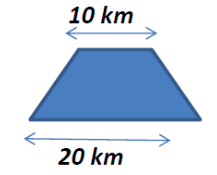
\includegraphics[scale=1]{cloud.png} 
\end{figure}\\

When this happens the production of solar power reduces by $ 90% $.

\begin{table}[H] 
\begin{tabular}{ll}
\toprule
Location & Power (MW) \\
\midrule
Brytpunkten & $ 96*0.1 = 9.6 MW$\\
Framtiden  &  $ 96*0.1 =  9.6 MW$\\
Solsidan & $ 96*0.1 =  9.6 MW$\\
\bottomrule
\end{tabular} 
\end{table} 

\begin{figure}[h] 
\label{powerchange}
\includegraphics[scale=0.5]{powerchange.png} 
\caption{Change of power with time in Solsidan (Blue), Framtiden and Brytpunkten (Red).}
\end{figure}\\


To calculate how much the frequency decreases with time when the cloud passes following formula is used,  
\begin{equation}
\Delta f = \Delta P /R
\end{equation}
Where $ \Delta f $ is the change in frequency, $ \Delta P =  86.4 MW $ is the change in power and $ R = 4300 MW/Hz $ is the gain. This results in the following graph, 

\begin{figure}[h] 
\label{frequency}
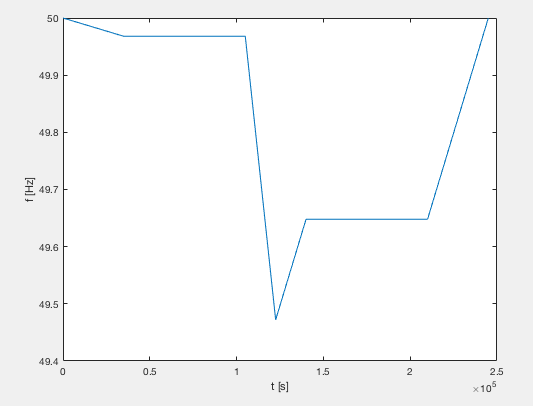
\includegraphics[scale=0.5]{frequency.png} 
\caption{Change of frequency with time.}
\end{figure}\\

The frequency starts at $ 50 Hz $ and goes down to $ 49.472 Hz $ when it is located over all three of the areas. 

\mypart{E}{How do we get more people interested in installing solar cells on their houses?}
One part of getting people interested in getting solar cells for their houses is knowledge. To get people interested in this they need to know that it is an option. It is also important to know why you should care about environmental questions and what solar cells got to do with this. How to get the solar cells and install them is important to know so that people don't think that it is harder that it actually is. A lot of the time just getting started with getting the necessary information is the hardest part. Once that part is covered the gain of having solar cells is important. One thing mentioned earlier in the report is subsidizing means such as tax reduction to get people to invest in solar cells is important. But the most important part is probably knowledge about solar cells. One way is to install more solar cells in public areas. When people notice the solar cells it can and interest in them. Solar cells can also inspire people to engage in other sustainable development questions. One example of this is the project "Ecostaden Augustenborg" in Malmö which inspired local schools to engage in  sustainable development questions and raised awareness and interest among children. (Naturvårdsverket, 2005) 
\end{document}

\chapter*{Introduction}
Naturvårdsverket, 2005. Att länka miljöeffekter och sociala effekter – en utvärdering av LIP-finansierade bostadsförnyelseprojekt. Jenny Stenberg och Liane Thuvander
https://www.naturvardsvproject erket.se/Documents/publikationer/620-5511-9.pdf\\

Nasdaq. 2017. MARKET PRICES. Nasdaq.
http://www.nasdaqomx.com/commodities/market-prices\\

European Energy Exchange. 2017. EU guideline 2009/28/EC on trading of Guarantees of Origin. European Energy Exchange.
https://www.eex.com/en/goo



